% Multi-panel figure for the Experiment-2 width tradeoff, generated by
% plot_experiment2_width_tradeoff.py. Requires \usepackage{graphicx} and
% \usepackage{subcaption}. Paths are relative to the repo root (Figs/...);
% adjust \graphicspath or the paths below to match the Overleaf project.
% Include with: % Multi-panel figure for the Experiment-2 width tradeoff, generated by
% plot_experiment2_width_tradeoff.py. Requires \usepackage{graphicx} and
% \usepackage{subcaption}. Paths are relative to the repo root (Figs/...);
% adjust \graphicspath or the paths below to match the Overleaf project.
% Include with: % Multi-panel figure for the Experiment-2 width tradeoff, generated by
% plot_experiment2_width_tradeoff.py. Requires \usepackage{graphicx} and
% \usepackage{subcaption}. Paths are relative to the repo root (Figs/...);
% adjust \graphicspath or the paths below to match the Overleaf project.
% Include with: % Multi-panel figure for the Experiment-2 width tradeoff, generated by
% plot_experiment2_width_tradeoff.py. Requires \usepackage{graphicx} and
% \usepackage{subcaption}. Paths are relative to the repo root (Figs/...);
% adjust \graphicspath or the paths below to match the Overleaf project.
% Include with: \input{experiment2_width_tradeoff_figure}
\begin{figure}[htbp]
\centering
\begin{subfigure}[t]{0.48\linewidth}
  \centering
  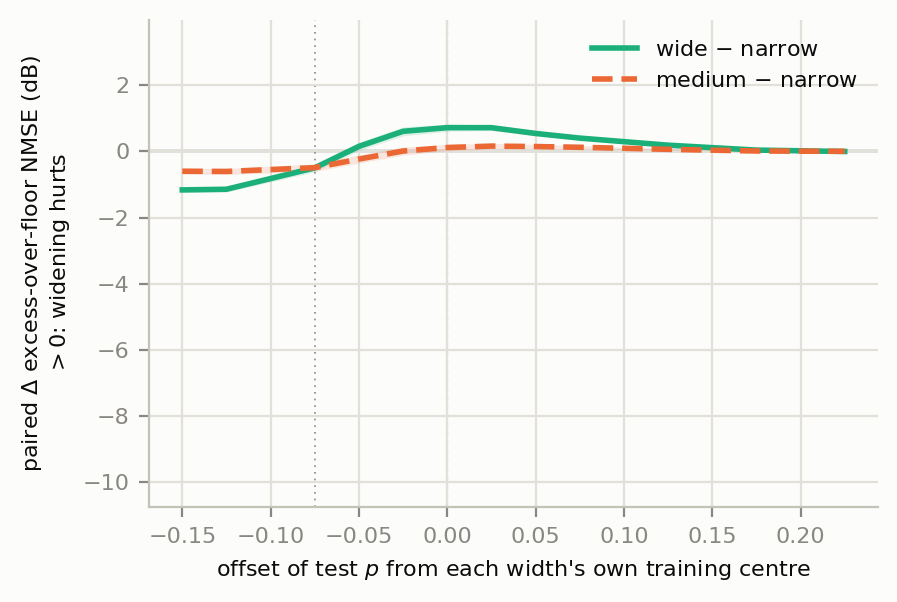
\includegraphics[width=\linewidth]{Figs/experiment2/width_tradeoff_nmse_exp2_try2_lista.png}
  \caption{LISTA, $(25,50)$, noiseless, centred widths (10 seeds)}
  \label{fig:exp2-width-tradeoff-exp2-try2-lista}
\end{subfigure}\hfill
\begin{subfigure}[t]{0.48\linewidth}
  \centering
  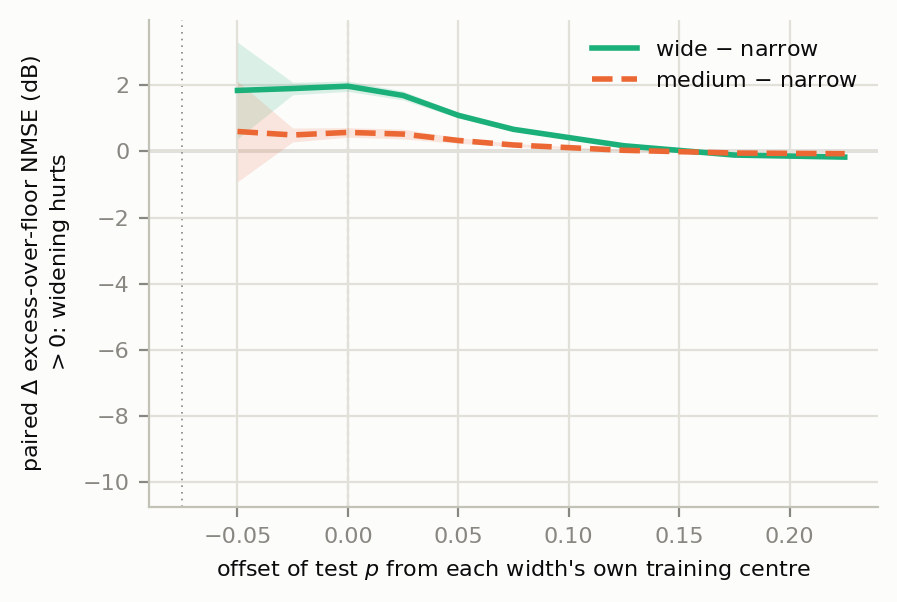
\includegraphics[width=\linewidth]{Figs/experiment2/width_tradeoff_nmse_exp2_try2_alista.png}
  \caption{ALISTA, $(25,50)$, noiseless, centred widths (10 seeds)}
  \label{fig:exp2-width-tradeoff-exp2-try2-alista}
\end{subfigure}\\[6pt]
\begin{subfigure}[t]{0.48\linewidth}
  \centering
  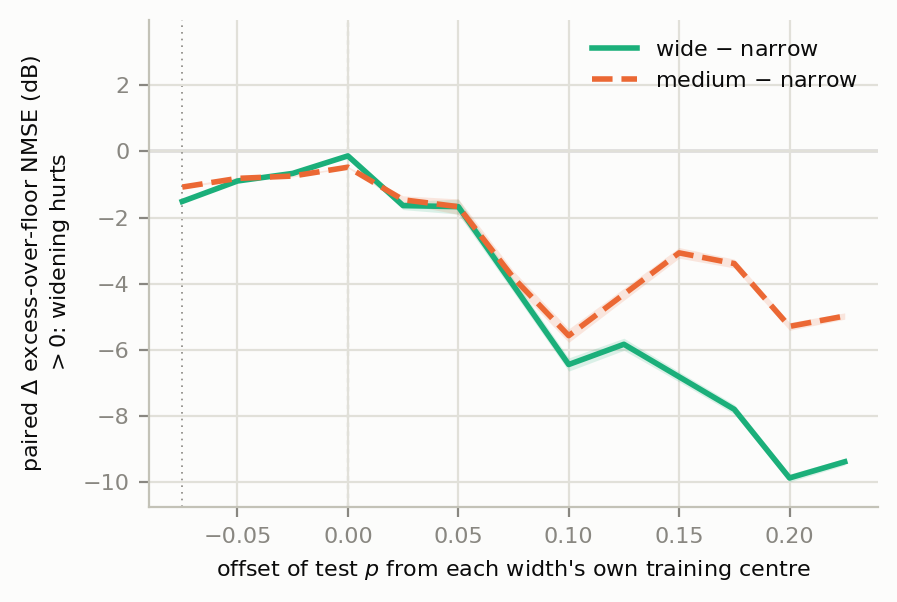
\includegraphics[width=\linewidth]{Figs/experiment2/width_tradeoff_nmse_exp2_real_lista.png}
  \caption{LISTA, $(210,300)$, SNR 40 dB, uncentred widths (10 seeds)}
  \label{fig:exp2-width-tradeoff-exp2-real-lista}
\end{subfigure}\hfill
\begin{subfigure}[t]{0.48\linewidth}
  \centering
  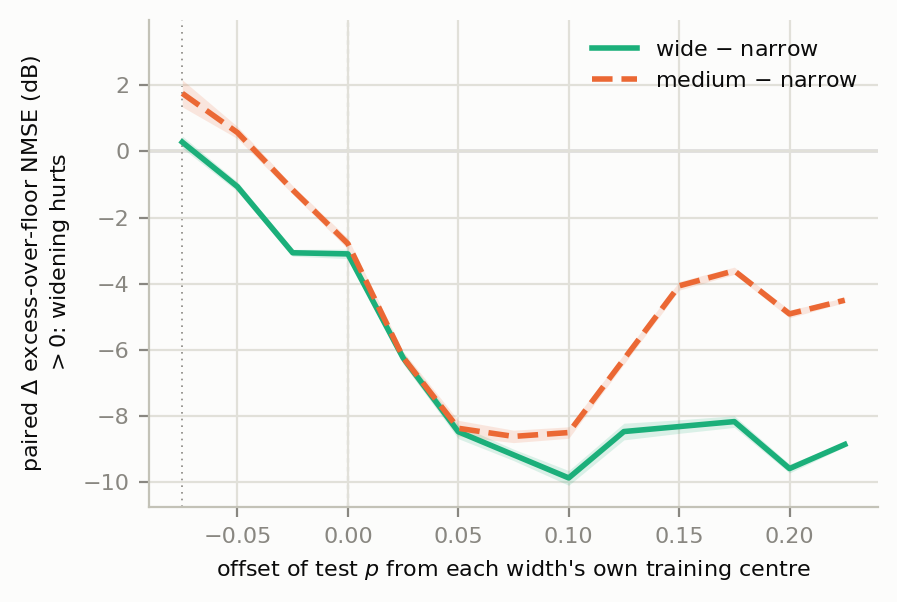
\includegraphics[width=\linewidth]{Figs/experiment2/width_tradeoff_nmse_exp2_real_alista.png}
  \caption{ALISTA, $(210,300)$, SNR 40 dB, uncentred widths (10 seeds)}
  \label{fig:exp2-width-tradeoff-exp2-real-alista}
\end{subfigure}\\[6pt]
\caption{Experiment 2: what widening the training-sparsity distribution costs in-distribution and buys out-of-distribution, for LISTA and ALISTA. Each curve is the mean over seeds of the paired difference (wide $-$ narrow, medium $-$ narrow) in excess-over-floor NMSE, i.e.\ NMSE vs.\ $x_\mathrm{true}$ minus the LASSO-optimal recovery error at the same test $p$, plotted against the offset of the test sparsity from each width's own training centre; bands are 95\% $t$-intervals over seeds. Positive values mean the wider training distribution is worse. The value at offset 0 is the in-distribution cost of widening; the curve relative to that value is the robustness benefit. Dotted verticals mark the offsets reported in Table~\ref{tab:exp2-width-tradeoff}. Points where a width is in the exact-recovery regime (raw NMSE below $-60$ dB) are omitted.}
\label{fig:exp2-width-tradeoff}
\end{figure}

\begin{figure}[htbp]
\centering
\begin{subfigure}[t]{0.48\linewidth}
  \centering
  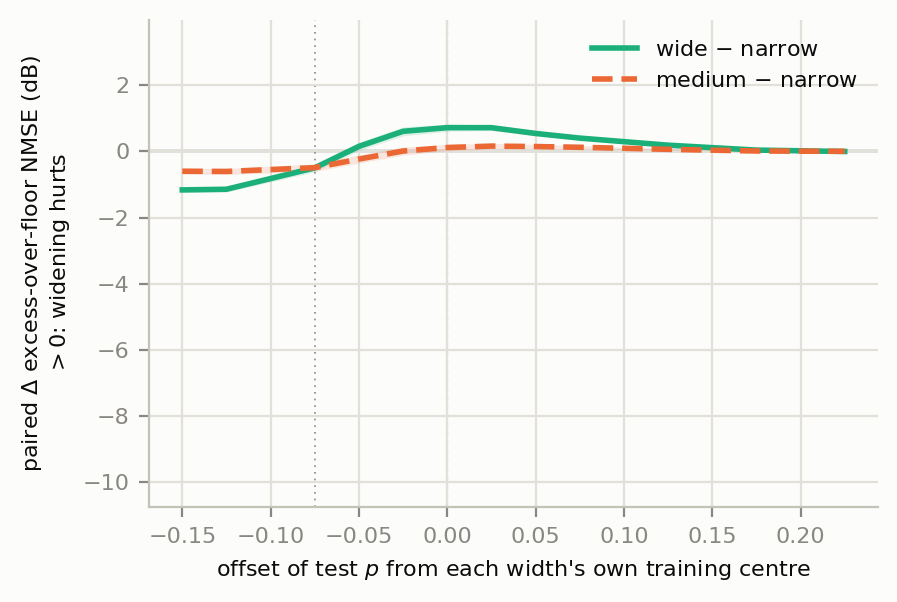
\includegraphics[width=\linewidth]{Figs/experiment2/width_tradeoff_nmse_exp2_try2_lista.png}
  \caption{LISTA, $(25,50)$, noiseless, centred widths (10 seeds)}
  \label{fig:exp2-width-tradeoff-exp2-try2-lista}
\end{subfigure}\hfill
\begin{subfigure}[t]{0.48\linewidth}
  \centering
  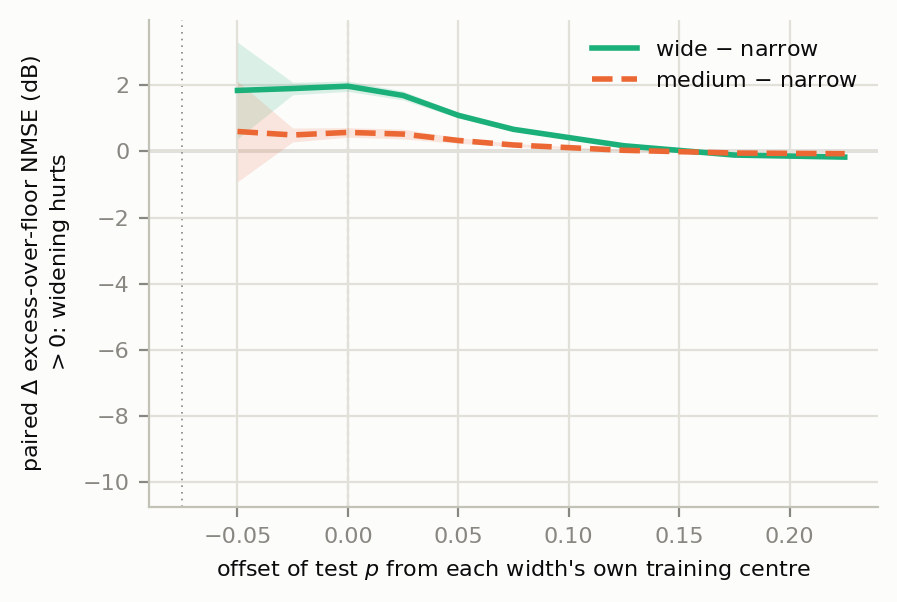
\includegraphics[width=\linewidth]{Figs/experiment2/width_tradeoff_nmse_exp2_try2_alista.png}
  \caption{ALISTA, $(25,50)$, noiseless, centred widths (10 seeds)}
  \label{fig:exp2-width-tradeoff-exp2-try2-alista}
\end{subfigure}\\[6pt]
\begin{subfigure}[t]{0.48\linewidth}
  \centering
  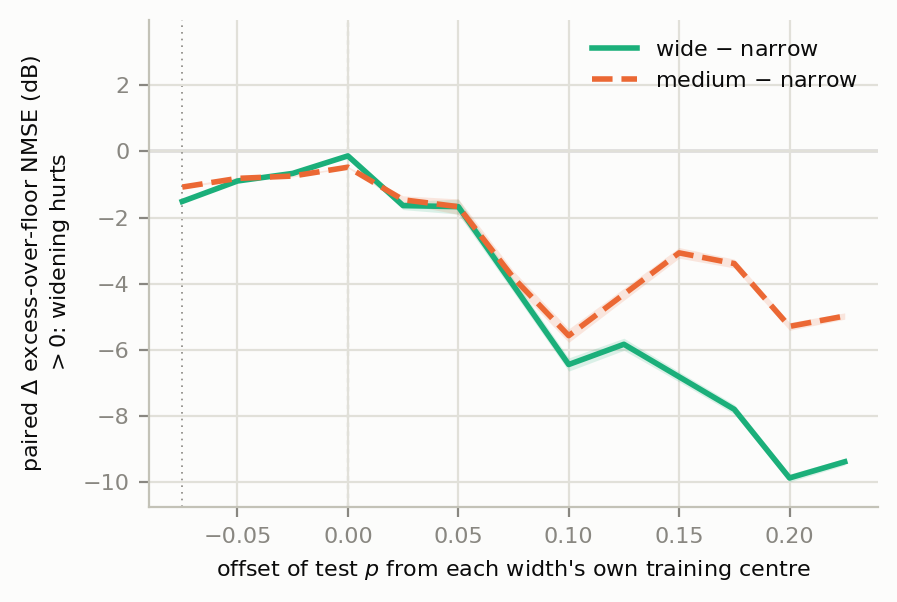
\includegraphics[width=\linewidth]{Figs/experiment2/width_tradeoff_nmse_exp2_real_lista.png}
  \caption{LISTA, $(210,300)$, SNR 40 dB, uncentred widths (10 seeds)}
  \label{fig:exp2-width-tradeoff-exp2-real-lista}
\end{subfigure}\hfill
\begin{subfigure}[t]{0.48\linewidth}
  \centering
  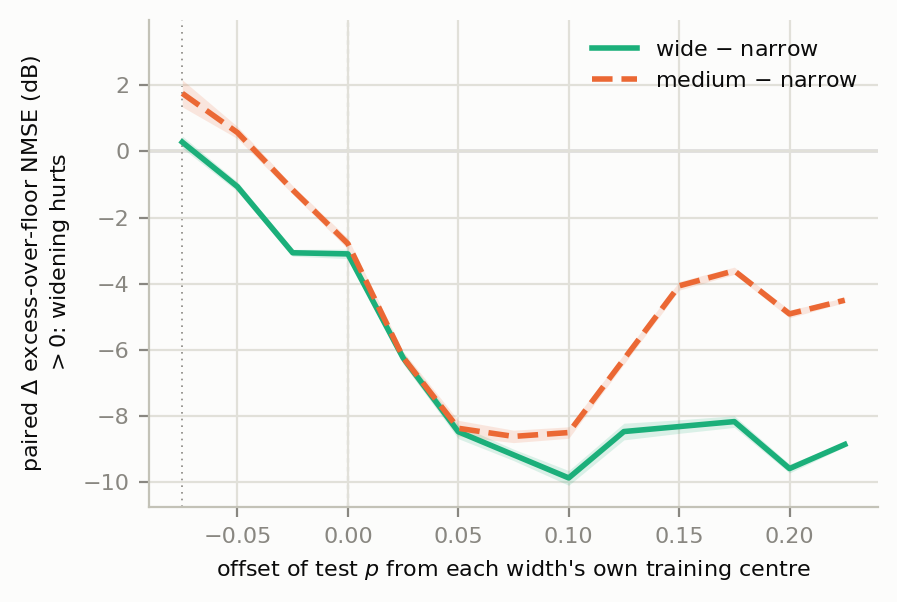
\includegraphics[width=\linewidth]{Figs/experiment2/width_tradeoff_nmse_exp2_real_alista.png}
  \caption{ALISTA, $(210,300)$, SNR 40 dB, uncentred widths (10 seeds)}
  \label{fig:exp2-width-tradeoff-exp2-real-alista}
\end{subfigure}\\[6pt]
\caption{Experiment 2: what widening the training-sparsity distribution costs in-distribution and buys out-of-distribution, for LISTA and ALISTA. Each curve is the mean over seeds of the paired difference (wide $-$ narrow, medium $-$ narrow) in excess-over-floor NMSE, i.e.\ NMSE vs.\ $x_\mathrm{true}$ minus the LASSO-optimal recovery error at the same test $p$, plotted against the offset of the test sparsity from each width's own training centre; bands are 95\% $t$-intervals over seeds. Positive values mean the wider training distribution is worse. The value at offset 0 is the in-distribution cost of widening; the curve relative to that value is the robustness benefit. Dotted verticals mark the offsets reported in Table~\ref{tab:exp2-width-tradeoff}. Points where a width is in the exact-recovery regime (raw NMSE below $-60$ dB) are omitted.}
\label{fig:exp2-width-tradeoff}
\end{figure}

\begin{figure}[htbp]
\centering
\begin{subfigure}[t]{0.48\linewidth}
  \centering
  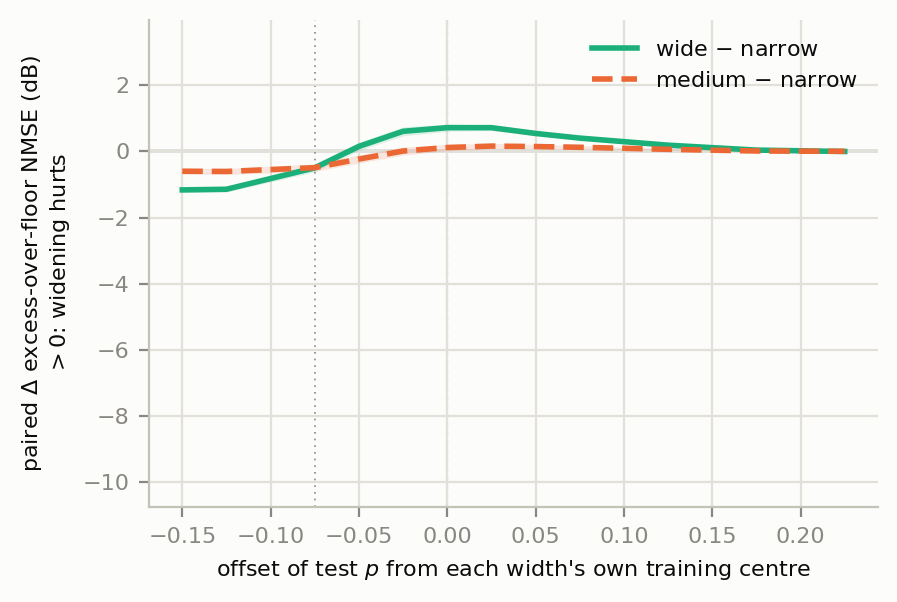
\includegraphics[width=\linewidth]{Figs/experiment2/width_tradeoff_nmse_exp2_try2_lista.png}
  \caption{LISTA, $(25,50)$, noiseless, centred widths (10 seeds)}
  \label{fig:exp2-width-tradeoff-exp2-try2-lista}
\end{subfigure}\hfill
\begin{subfigure}[t]{0.48\linewidth}
  \centering
  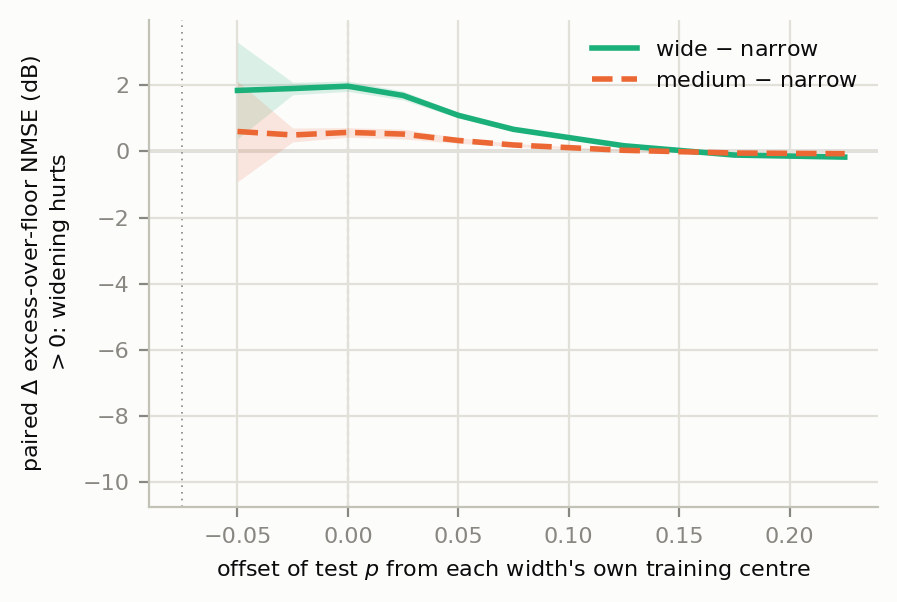
\includegraphics[width=\linewidth]{Figs/experiment2/width_tradeoff_nmse_exp2_try2_alista.png}
  \caption{ALISTA, $(25,50)$, noiseless, centred widths (10 seeds)}
  \label{fig:exp2-width-tradeoff-exp2-try2-alista}
\end{subfigure}\\[6pt]
\begin{subfigure}[t]{0.48\linewidth}
  \centering
  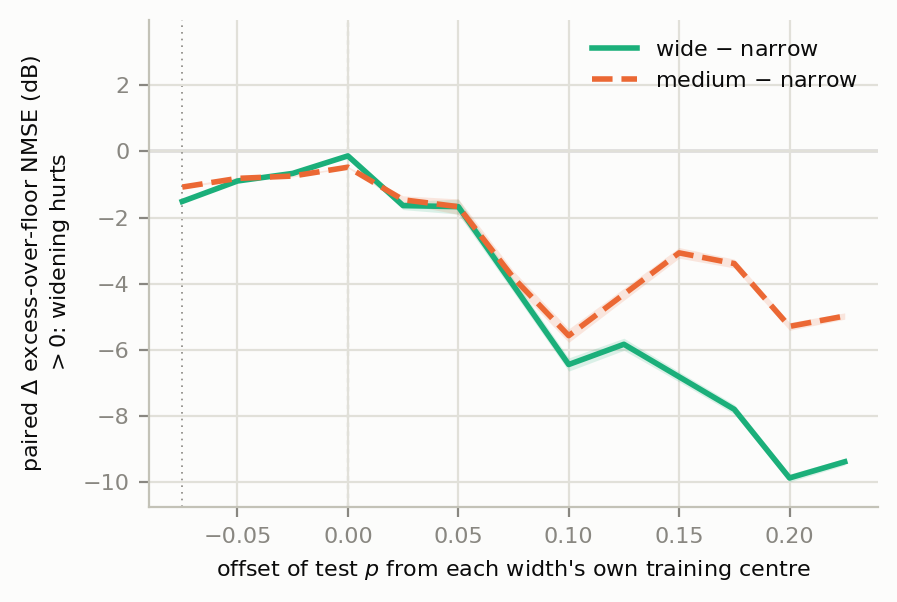
\includegraphics[width=\linewidth]{Figs/experiment2/width_tradeoff_nmse_exp2_real_lista.png}
  \caption{LISTA, $(210,300)$, SNR 40 dB, uncentred widths (10 seeds)}
  \label{fig:exp2-width-tradeoff-exp2-real-lista}
\end{subfigure}\hfill
\begin{subfigure}[t]{0.48\linewidth}
  \centering
  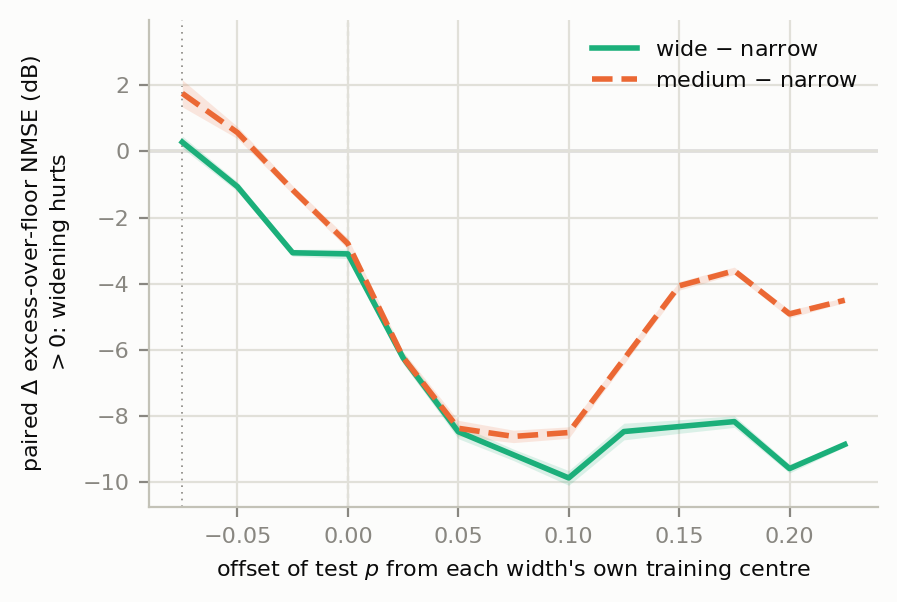
\includegraphics[width=\linewidth]{Figs/experiment2/width_tradeoff_nmse_exp2_real_alista.png}
  \caption{ALISTA, $(210,300)$, SNR 40 dB, uncentred widths (10 seeds)}
  \label{fig:exp2-width-tradeoff-exp2-real-alista}
\end{subfigure}\\[6pt]
\caption{Experiment 2: what widening the training-sparsity distribution costs in-distribution and buys out-of-distribution, for LISTA and ALISTA. Each curve is the mean over seeds of the paired difference (wide $-$ narrow, medium $-$ narrow) in excess-over-floor NMSE, i.e.\ NMSE vs.\ $x_\mathrm{true}$ minus the LASSO-optimal recovery error at the same test $p$, plotted against the offset of the test sparsity from each width's own training centre; bands are 95\% $t$-intervals over seeds. Positive values mean the wider training distribution is worse. The value at offset 0 is the in-distribution cost of widening; the curve relative to that value is the robustness benefit. Dotted verticals mark the offsets reported in Table~\ref{tab:exp2-width-tradeoff}. Points where a width is in the exact-recovery regime (raw NMSE below $-60$ dB) are omitted.}
\label{fig:exp2-width-tradeoff}
\end{figure}

\begin{figure}[htbp]
\centering
\begin{subfigure}[t]{0.48\linewidth}
  \centering
  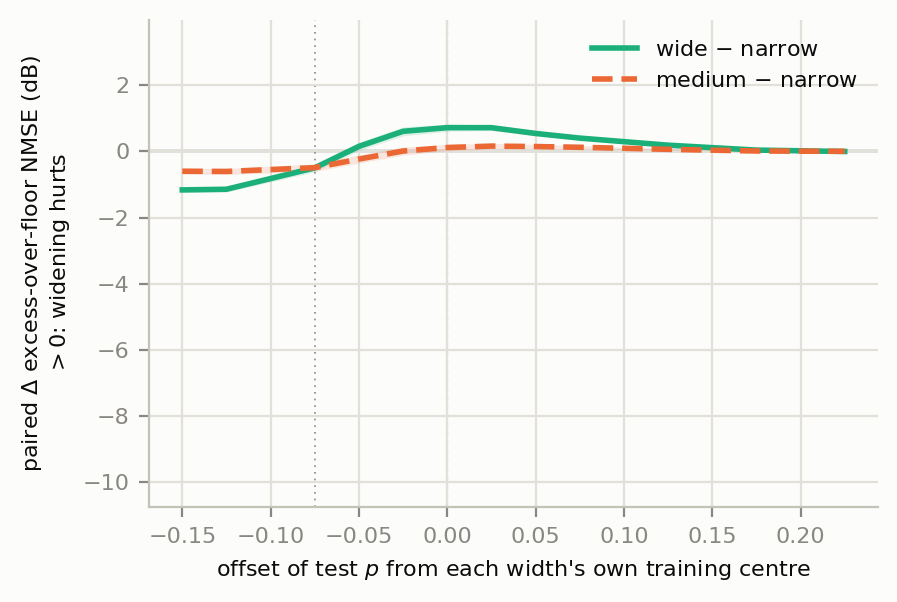
\includegraphics[width=\linewidth]{Figs/experiment2/width_tradeoff_nmse_exp2_try2_lista.png}
  \caption{LISTA, $(25,50)$, noiseless, centred widths (10 seeds)}
  \label{fig:exp2-width-tradeoff-exp2-try2-lista}
\end{subfigure}\hfill
\begin{subfigure}[t]{0.48\linewidth}
  \centering
  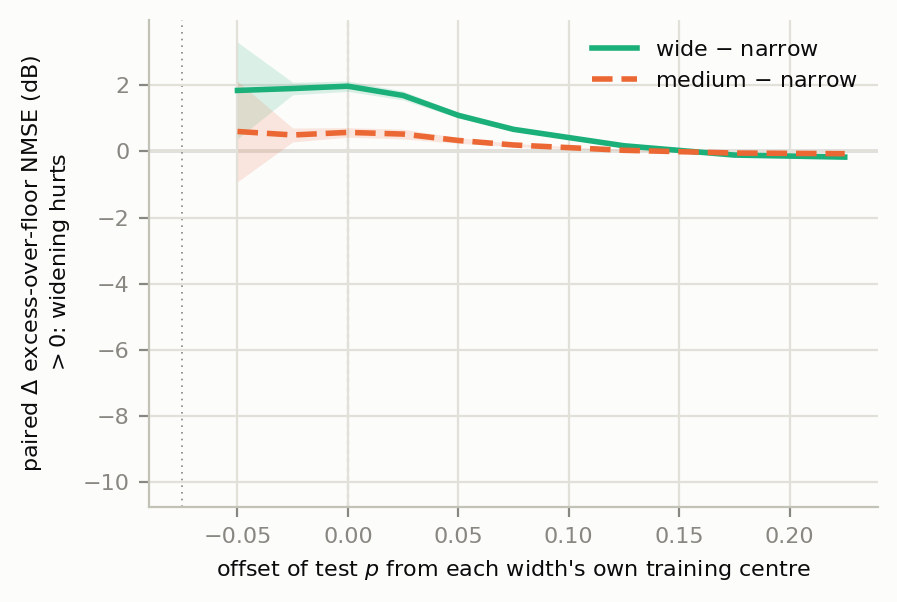
\includegraphics[width=\linewidth]{Figs/experiment2/width_tradeoff_nmse_exp2_try2_alista.png}
  \caption{ALISTA, $(25,50)$, noiseless, centred widths (10 seeds)}
  \label{fig:exp2-width-tradeoff-exp2-try2-alista}
\end{subfigure}\\[6pt]
\begin{subfigure}[t]{0.48\linewidth}
  \centering
  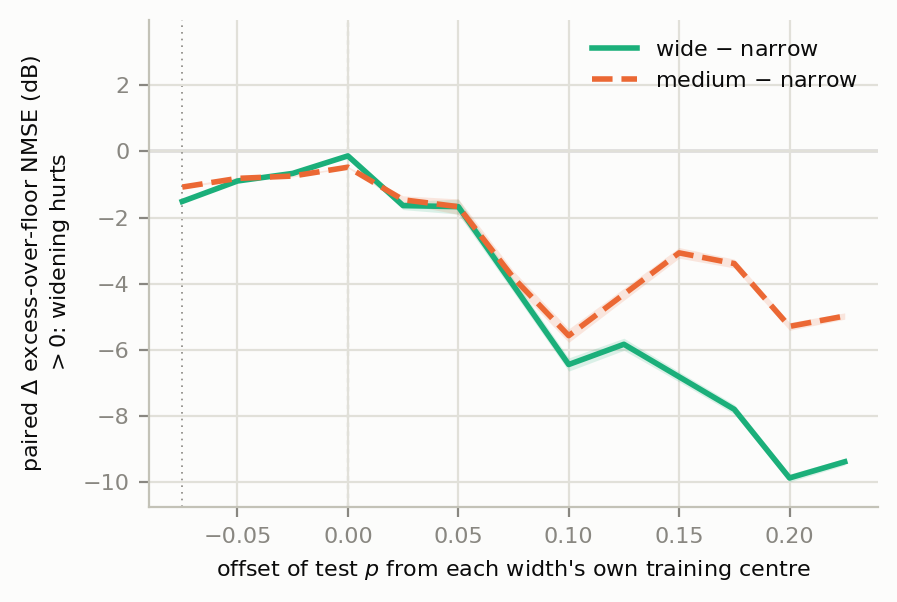
\includegraphics[width=\linewidth]{Figs/experiment2/width_tradeoff_nmse_exp2_real_lista.png}
  \caption{LISTA, $(210,300)$, SNR 40 dB, uncentred widths (10 seeds)}
  \label{fig:exp2-width-tradeoff-exp2-real-lista}
\end{subfigure}\hfill
\begin{subfigure}[t]{0.48\linewidth}
  \centering
  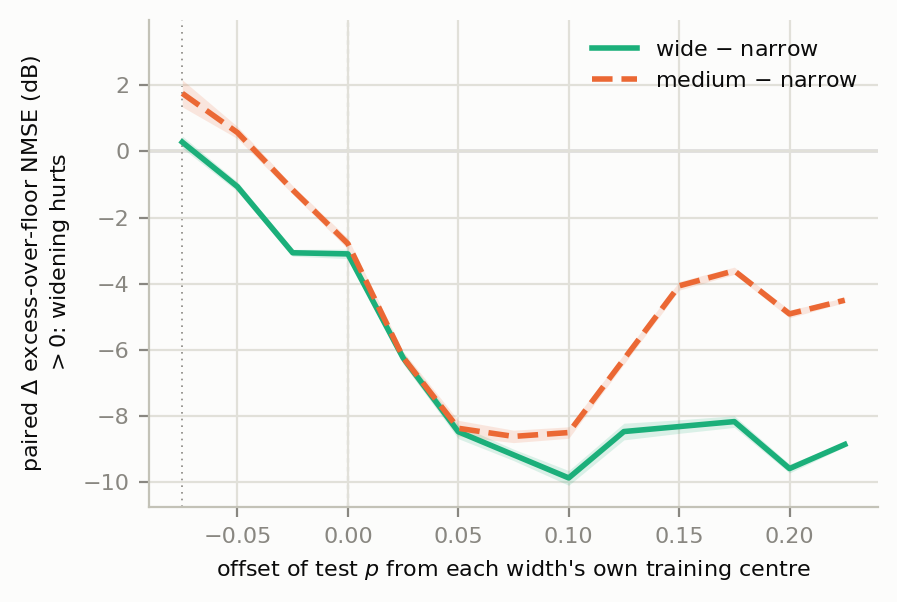
\includegraphics[width=\linewidth]{Figs/experiment2/width_tradeoff_nmse_exp2_real_alista.png}
  \caption{ALISTA, $(210,300)$, SNR 40 dB, uncentred widths (10 seeds)}
  \label{fig:exp2-width-tradeoff-exp2-real-alista}
\end{subfigure}\\[6pt]
\caption{Experiment 2: what widening the training-sparsity distribution costs in-distribution and buys out-of-distribution, for LISTA and ALISTA. Each curve is the mean over seeds of the paired difference (wide $-$ narrow, medium $-$ narrow) in excess-over-floor NMSE, i.e.\ NMSE vs.\ $x_\mathrm{true}$ minus the LASSO-optimal recovery error at the same test $p$, plotted against the offset of the test sparsity from each width's own training centre; bands are 95\% $t$-intervals over seeds. Positive values mean the wider training distribution is worse. The value at offset 0 is the in-distribution cost of widening; the curve relative to that value is the robustness benefit. Dotted verticals mark the offsets reported in Table~\ref{tab:exp2-width-tradeoff}. Points where a width is in the exact-recovery regime (raw NMSE below $-60$ dB) are omitted.}
\label{fig:exp2-width-tradeoff}
\end{figure}
